\chap{"Hai, Engkau Betlehem..."}
\small 

\begin{wrapfigure}{l}{2.2cm}
\centering
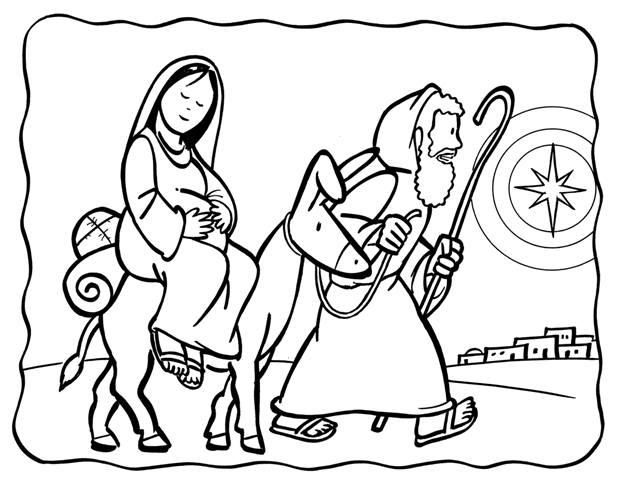
\includegraphics[scale=1]{gambar/11.jpg}
\end{wrapfigure}


\noindent{Adalah utang tetapi mustahil melunasinya namun, merupakan kekayaan dan kenangan paling berharga yang telah memaknai dan mengarisbawahi batin dan hati setiap peziarah ke Tanah Suci yang sampai sekarang masih diperdebatkan oleh Palestina dan Israel. }

Adalah satu pengalaman yang sulit untuk dilupakannya. Pengalaman pribadiku membisikan ketidakpercayaan bahwa suatu saat aku akan mengunjungi Tanah Suci. Aku tidak pernah memimpikannya, apalagi mengharapkan dan merencanakan untuk mengunjunginya. Namun Allah sendiri telah merencanakan sesuatu yang sama sekali berlainan dengan rencanaku. Oleh karena rahmat dan pengutusanNya, aku berhutang padaNya. Apa yang semestinya aku lakukan? Meskipun aku berniat untuk melakukan sesuatu tindakan bagiNya, tentu masih saja tidak berarti. Namun, setidaknya aku mencoba untuk mengoreskan pengalamanku ini kepada orang lain selagi aku bisa.

Betlehem adalah tempat bersejarah yang paling dekat dengan komunitas salesian di Cremisan yang hanya bisa ditempuh kurang lebih $\frac{1}{4}$ jam dengan kendaraan pribadi atau umum. Biasanya para frater memilih alternatif lain untuk mengapainya yaitu berjalan kaki. Merupakan tempat bersejarah pertama yang aku kunjungi ketika baru pertama kali aku menginjakan kakiku di Tanah Suci. Seseorang bisa saja bertanya, apa emosi anda? Tentu saja lain dari yang lain. Emosi setiap orang adalah subyektif. Percaya atau tidak bukanlah permasalahan kita sekarang. Penting adalah bagaimana seseorang dihadapan pada suatu realitas yang selama ini tersembunyi di bawah kemisterian. Artinya, nama Betlehem hanya menjadi sebuah cerita belaka. Selebihnya aku bukan dihadapan pada sebuah misteri tersembunyi. Aku menyentuhnya dengan tanganku sendiri dan mengawasinya dengan mataku sendiri secara seksama. Dan bagaimana gua ini terpelihara hingga sekarang? Merupakan pertanyaan setiap orang, baik bagi mereka yang telah mengunjunginya ataupun bagi mereka-mereka yang hanya mendengar namanya saja. 

Betlehem, adalah nama yang mengekspresikan misteri kemenangan dalam kemiskinan; kemiskinan Bunda Maria dan Santu Yosep namun, kemiskinan mereka diterangi oleh kemenangan Natal dengan kelahiran sang Terang, Yesus Kristus. Terang itu menerangi semua orang di planet bumi ini, menerangi hati dan budi setiap orang yang mencari Allah, seperti terjadi pada orang-orang Majus dari Timur. Terang itu membawa mereka menemukan Yesus seperti yang mereka masing-masing mengharapkannya. Kehadiran Yesus ini adalah sebagai Allah Pembawa damai bagi para umatNya.

Betlehem, dalam bahasa Yahudi, "Rumah Roti" dan dalam bahasa Arab, "Rumah Daging", terletak di pinggir padang gurun yang dalam Kitab Suci dikenal sebagai EFRATA (artinya yang mengandung buah, yang berbuah); berpenduduk sekitar 40.000 orang, mayoritas orang Arab, baik kristiani maupun Islam.

Betlehem adalah satu daerah yang dirahmati dengan beraneka macam kekayaan. Rumah-rumahnya berbatu putih mengkilat, dikelilingi dengan sekelompok besar kawanan domba, yang menciri-khaskan tradisi setempat; dikelilingi juga oleh lahan dengan tanaman zaitun. Dari kesemuanya ini di hadapan pandangan mata kita bagaikan sebuah palungan alamiah yang indah. 

Pada zaman Yesus, meskipun Yehuda adalah termasuk bagian kekuasaan raja Daud, Betlehem tetaplah merupakan sebuah kota kecil tak dikenal di antara kota-kota lain disekitarnya. Keadaan geografisnya tidak menguntungkan untuk menemukan kembali letak kestrategisannya atau kepolitikkannya. Namun, bagaimanapun juga tidak disangkal nama Betlehem pada saat ini termashyur, dikagumi untuk sepanjang dan segala masa. 

Pada zamannya nabi Mikha, ia memprofesikan kemashyuran kota kecil Betlehem, dengan bernubuat:"Engkau, hai Betlehem Efrata, hai yang terkecil di antara kaum-kaum Yehuda, dari padamu akan bangkit bagiKu seorang yang akan memerintah Israel, yang permulaannya sudah sejak purbakala, sejak dahulu kala" (Mi, 5,1).

Di jantung Basilika yang akrabnya dipanggil Basilika Kelahiran Yesus terdapat gua atau kandang domba kelahiran Yesus. Basilika ini merupakan yang tertua di antara semua basilika atau gereja di dunia. Alasannya sederhana: karena merupakan Basilika pertama di Tanah Suci yang memancarkan gua mistik dimana Yesus dilahirkan. Dan selanjutnya menjadi tempat kudus bagi orang-orang Kristen pertama, dan merupakan pusat penghormatan kekudusan Allah. 

Kesaksian sejarah menceritakan bahwa pada zaman Kaisar Adrianus, sekitar tahun 135 setelah Kristus, ia menghendaki agar menghapuskan dari semua tempat kudus lambang-lambang kesucian Kristiani. Begitupun dengan Yerusalem, dimana ia memerintahkan untuk meratakan puncak Golgota, dengan membangunkannya kembali di atas sebuah bangunan untuk memberi penghormatan kepada para dewa-dewi. Di Betlehem, seperti dikisahkan bahwa Gua kelahiran Yesus ini pada awalnya telah disembunyikan dengan timbunan tanah, dan diatasnya ditanamkan sekelompok tanaman hijau, dimana menjadikan Gua kelahiran Yesus ini menjadi sebuah hutan rimba suci bagi dewa kesuburan.

Namun, keprofananya tidak berlangsung lama. Selang waktu sebelum berakhirnya zaman kepahitan itu, gua kelahiran Yesus digunakannya kembali oleh orang-orang kristiani untuk berdoa, adorasi dan sebagainya.
Dari tahun 215, tradisi mengkisahkan juga bahwa kesaksian filsuf dan teolog Origene menunjukkan bahwa Gua itu merupakan tempat kelahiran Penyelamat dunia dan kandang para kawanan domba. Fakta ini membuktikan adanya keaslian. Begitupun sesuai dengan kesaksian orang-orang disekitarnya baik yang percaya maupun yang tidak percaya kepada Allah pada zaman itu.

Pada tahun 325, ibu Kaisar Kostantino, memberikan kepada orang kristen kebebasan untuk beribadat. Maka, Kostantino memulai untuk membangun di atas Gua itu sebuah Basilika. Basilika tertua ini masih terlihat hingga sekarang.

Pada tahun 384, Santo Hieronimus memilih untuk mendirikan di dekat gua ini, sebuah komunitas religius. Orang kudus ini, membaktikan hampir setengah dari hidup kebiaraannya, kurang lebih selama 36 tahun dengan kehidupan berdoa dan menerjemahan Kitab Suci dari bahasa Ibrani dan Yunani ke dalam bahasa Latin; kesaksiannya mengisahkan bahwa: "Hai! Betapa baiknya, seandainya aku dianugerahkan rahmat untuk melihat sendiri keaslian kandang kelahiran dimana Bayi Yesus dilahirkan dan diletakkan! Namun, hanya untuk sebuah venerasi saja, kita telah meniadakan keaslian kandangnya dengan membangunkannya kembali sebuah gua atau kandang berlapiskan marmer. Seberapa harganyakah bagiku semuanya ini? Apa gunanya semuanya ini bagiku?"

Pada tahun 531, Kaisar Yustinianus memperbaikinya lagi bangunan ini yang telah didirikan atas perintah Santa Helena, ibu Kaisar Kostantino. Yustinianus mencoba mengkostruksikannya lagi bangunan ini dengan mempertahankan keasliannya tanpa merubah bentuk keasliannya. Karena bangunan ini telah terukir banyak sejarah, terutama bertahannya terhadap serangan-serangan dari luar seperti dari serangan orang-orang Islam pada umumnya.

Pintu masuk Basilika yang sekarang berukuran sangat kecil; yang tingginya kurang lebih 1 meter dan lebarnya 45 centimeter. Tiga buah pintu lainnya terpaksa ditutup untuk menghindari masuknya para tentara Otomani dengan berkuda. Pintu masuk yang ada hinga sekarang ini sangat rendah ketinggiannya merupakan sebuah kenangan terbaik yang bisa memaknai ingatan budi setiap peziarah. Melambangkan ketidaklayakan manusia di hadapan kemahakuasaan Allah.

\section*{Di gua bersama MARIA}

Tampaknya menjadi sesuatu yang biasa. Bagi siapa yang masuk ke dalam Basilika pertanyaannya yang pertama adalah "dimanakah gua itu"? Gua merupakan pusat dan hati dari basilika. Gua ini dipancarkan dengan sebuah bintang beremaskan perak, dengan tulisan:"di sini, oleh Bunda Maria Yesus dilahirkan". Dengan demikian, pusat perhatian kita di dalam gua itu tertuju pada cahaya tersebut. Para peziarah berlutut dan mencium bintang bersahaja itu. Adalah Misteri cintakasih Allah! Allah dengan bahasa sederhananya, mewahyukan diriNya, menjadikan diriNya visibil, terjangkau, dalam bentuk seorang manusia: "Maria melahirkan seorang anak laki-laki, lalu dibungkusnya sengan lapin dan dibaringkannya di dalam palungan, karena tidak ada tempat bagi mereka di rumah penginapan"(Luk. 2,7). 

Renungkanlah sesaat. Seperti ibu-ibu yang lain, Maria pada saat itu, rupanya sedikit sibuk untuk menamai sang kecil. Maria mulai berbisik kepada sang kecil, tanpa nama itu: "hai bunga kecilku, nama apa yang selayaknya kuberikan untukmu?" Seorang manusia? Tetapi kandunganMu adalah Kudus Ilahi. Engkaukah Tuhan? Tetapi, Engkau mengambil rupa manusia. Jadi, apa yang hendak kuperbuat bagimu? Engkau akan kususui atau dihormati sebagai Yang Kudus, Allah? Akankah kupelihara atau diperlakukan sebagai seorang hamba"?

Ataukah hanya sekedar bahwa pada saat itu, tidak ada tempat penginapan lagi bagi mereka. Ataukah dilahirkan sebagai yang terakhir dari generasi manusia, tanpa rumah pernginapan, tak mempunyai apa-apa. Jawaban yang semestinya diberikan kepadaNya adalah: "Terang itu bercahaya di dalam kegelapan dan orang tidak menerimaNya... Ia datang kepada milik kepunyaanNya, tetapi orang-orang kepunyaanNya itu tidak menerimaNya" (Yoh.1,5-11). 

Pesan Natal, yang seharusnya kita berikan pada setiap perayaan Natal, bukan yang lain selain: "MENERIMA KRISTUS".

Setelah 2000 tahun berlalu, tempat penginapan apa yang kita buatkan untuk Yesus??? Seharusnya kita membuatkan tempat penginapan bagiNya; tempatNya adalah di dalam hati dunia dan hati setiap orang. Karena jika Dia telah menemukan tempat diantara kita dengan cintaNya; dan jika sampai sekarang ini, Dia masih mencari sesuatu dari kita bukan karena Dia menginginkanNya, tetapi demi keselamatan kita, maka seharusnya kita memenuhinya dengan bertumbuh dan lahir dari dalam (hati kita), tanpa harus seseorang yang memanuver, yakni CINTA KASIH.	

Allah (Yesus) telah menjawab "YA" kepada dunia: Manusia seharusnya juga menjawabnya "YA" kepada Allah. Karena itu merupakan satu-satunya kondisi atau jalan untuk memperoleh keselamatan: "tetapi semua orang yang menerimaNya diberiNya kuasa supaya menjadi anak-anak Allah, yaitu mereka yang percaya dalam namaNya"(Yoh.1,12). 

\sumber{Oleh: Fr. Acacio D. De Castro, SDB - Yerusalem \\email: addecastro@yahoo.co.uk}
\normalsize